\chapter{Deep Learning \& Automatic Differentiation}
\refb{Additional Resources}{

    \begin{itemize}
        \item \href{https://www.amazon.co.uk/gp/product/110845514X}{Automatic Differentiation, Section 5.6 (page 159) Deisenroth et al. (2020)}.
        \item \href{https://jingnanshi.com/blog/autodiff.html}{Online resource with implementation in Rust}.
        \item \href{https://www.youtube.com/watch?v=wG_nF1awSSY}{A polished video walk through of automatic differentiation}.
    \end{itemize}

}


\section{From GLMs to Multi-Layer Perceptrons}
Previously we saw that for generlaised linear models, which are only slightly more complex than neural networks, do not have a closed-form solution for finding the optimal parameters (unlike something like linear regression). Recall the generalised linear model (GLM) is given by:

\begin{equation}
    \bm{y} = \sigma(\theta^T \bm{x})
\end{equation}

where $\sigma$ is the link function, previously denoted as $g$. We perform basis expansion and use summation notation to represent the model as:

\begin{equation}
    \bm{y} = \sigma\left(\sum_{i=1}^n \theta_i x_i\right)
\end{equation}

This is the model of a single perceptron. A 2-D example is visualised in Figure \ref{fig:perceptron}.

\tikzset{
    neuron/.style={circle, draw, minimum size=1cm},
    input neuron/.style={neuron, fill=gray!20},
    output neuron/.style={neuron, fill=gray!60},
    activation function/.style={
            circle,
            draw,
            minimum size=1cm,
            fill=gray!30,
            path picture={
                    % Make sigma larger using \scalebox
                    \node at (path picture bounding box.center) {\scalebox{2.0}{$\Sigma$}}; % Scales sigma to 2x size
                }
        },
    arrow label/.style={midway, above}
}


\begin{marginfigure}
    \begin{tikzpicture}[>=Stealth, node distance=1.5cm, scale=0.6]
        % OR Perceptron
        \node[input neuron] (input1) {$1$};
        \node[input neuron, below of=input1] (inputx1) {$x_1$};
        \node[input neuron, below of=inputx1] (inputx2) {$x_2$};

        % Activation function with sigma inside
        \node[activation function, right of=inputx1] (activation1) {};

        \node[output neuron, right=0.75cm of activation1] (output1) {\scalebox{2.0}{$\sigma$}};
        \draw[->] (activation1) -- (output1);

        % \node[right=0.1cm of output1] (or) {OR$(x_1, x_2)$};

        % Arrows with weights
        \draw[->] (input1) -- (activation1) node[midway,above] {$b$};
        \draw[->] (inputx1) -- (activation1) node[midway,above] {$\theta_1$};
        \draw[->] (inputx2) -- (activation1) node[midway,above] {$\theta_2$};

        % Small arrow pointing right out of output node
        \draw[->] (output1) -- +(2, 0);
    \end{tikzpicture}
    \caption{A single perceptron.}
    \label{fig:perceptron}
\end{marginfigure}


\bigskip

Now to expand this to a network of multiple perceptrons, we remove the summation notation to add another perceptron:

\[
    [y_0, y_1] = \left[ \sigma(b_0 + \theta_0^\top \bm{x}), \sigma(b_1 + \theta_1^\top \bm{x}) \right]
\]

Notice how we now have a second output related to the same input. It then makes more sense to combine the parameter vectors $\theta_0$ and $\theta_1$ into a matrix $\theta := [\theta_0, \theta_1]$. This allows us to write the model as:

\[
    \bm{y} = \sigma(\theta^\top \bm{x})
\]

Where $\theta$ is a matrix of parameters, $\bm{y} \in \RR^2$ is the output vector, and $\bm{x} \in \RR^n$ is the input vector.


\subsection{The Single-Layer Perceptron}

We have previously discussed the $n$-dimensional generalisation of the generalised linear model (GLM). This model can now be viewed as a network of neurons. A matrix of size $m \times n$ represents the weighted connections in a bipartite graph on $m+n$ nodes, where each entry $i, j$ of the matrix represents the "strength" of the connection between node $i$ (the $i$th input dimension) and node $j$ (the $j$th output dimension).


By denoting the parameter matrix $\bm{W} \in \mathbb{R}^{m \times n}$, we can define the multi-layer perceptron as an extension of the GLM:

\[
    y = g^{-1} \left( \theta^\top \sigma (\bm{W} \bm{x} + \bm{b}) \right)
\]

To clarify, we break this into two stages, highlighting that $\theta \in \mathbb{R}^{m \times 1}$:

\begin{align}
    z & = \sigma (\bm{W} \bm{x} + \bm{b}) \label{eq:mlp1}     \\
    y & = g^{-1} \left( \theta^\top z \right) \label{eq:mlp2}
\end{align}

\begin{itemize}
    \item The first stage, Equation \ref{eq:mlp1}, represents the hidden neurons in the bipartite graph with weights $\bm{W}$.
    \item The second stage, Equation \ref{eq:mlp2}, maps the hidden layer of $m$ dimensions to the output space, forming another bipartite graph with weights determined by $\theta$.
\end{itemize}


\begin{figure*}[h!]
    \begin{tikzpicture}[every node/.style={draw, circle, minimum size=5mm, inner sep=1pt},
        >={Stealth}, shorten >=1pt]

        % Input vector
        \node[draw=none] (x1) at (0.2, 2.2) {} ; %{$x_1$};
        \node[draw=none] (x2) at (0.2, 1.75) {} ; %{$x_2$};
        \node[draw=none] (xn) at (0.2, 0.55) {} ; %{$x_n$};
        \node[draw=none] (b) at (0.2, 0.15) {} ;

        % \node[draw=none] (dots1) at (0, 0.75) {$\vdots$};
        \node[draw=none] (x) at (0, 1.25) {$\begin{bmatrix}
                    {x_1} \\ {x_2} \\ \vdots \\ {x_n} \\ 1
                \end{bmatrix}$};

        \node[draw=none] (theta) at (5.5, 4) {$\begin{bmatrix}
                    \theta_{1,1} \\
                    \theta_{2,1} \\
                    \vdots       \\
                    \theta_{n,1} \\
                    b_1
                \end{bmatrix}$};


        % Bracket for the input vector
        % \draw[thick] (-0.5, 3) -- (-0.5, -0.5);
        % \draw[thick] (-0.5, 3) -- (0.5, 3);
        % \draw[thick] (-0.5, -0.5) -- (0.5, -0.5);

        % Summation nodes
        \node (sum1) at (3, 3) {$\sum$};
        \node (sum2) at (3, 1.7) {$\sum$};
        \node (sum3) at (3, 0) {$\sum$};

        % Dots between summation nodes
        \node[draw=none] (dots2) at (3, 0.7) {$\vdots$};

        % Activation function node
        \node (sigma1) at (6, 1.5) {$\sigma$};

        % Output arrow
        \draw[->] (sigma1) -- +(0.65, 0) node[draw=none, right] {};

        \node[draw=none] (matrix-vector) at (3.2, 3.5) {$\sum_i \mb{x}_i \theta_{i,1}^{(1)} + b_1$};
        \node[draw=none] (matrix-vector) at (3.2, 1.2) {$\sum_i \mb{x}_i \theta_{i,2}^{(1)} + b_2$};
        \node[draw=none] (matrix-vector) at (3.2, -0.5) {$\sum_i \mb{x}_i \theta_{i,j}^{(1)} + b_j$};

        \node[draw=none, align=center] (matrix-vector) at (3.2, -1.6) {$\overbrace{\sum_i \underbrace{\mb{W}_{i,j}^{(1)}}_{K \times n} \underbrace{\mb{x}_{i}}_{n \times 1} }+\underbrace{ \mb{b}^{(1)}}_{k \times 1}$\\$ = \mb{W}^{(1)}x  + \mb{b}^{(1)}$};

        \node [draw=none](label) at (3.2, -3) {$j$ perceptrons in level (1)};

        % Arrows from input vector to summation nodes
        \foreach \i in {x1,x2,xn, b} {
                \draw[->] (\i.east) -- (sum1.west);
                \draw[->] (\i.east) -- (sum2.west);
                \draw[->] (\i.east) -- (sum3.west);
            }

        % Arrows from summation nodes to activation function
        \draw[->] (sum1.east) -- (sigma1.west);
        \draw[->] (sum2.east) -- (sigma1.west);
        \draw[->] (sum3.east) -- (sigma1.west);

        \draw[dashed, ->] (5.1,3.3) -- (sum1.east);


        % Dots between summation nodes
        \node[draw=none] (dots2) at (3, 0.7) {$\vdots$};


        % Output arrow
        % \draw[->] (sigma2) -- +(1, 0) ;

        % z vector
        \node[draw=none] (z1) at (7.2, 2) {};
        \node[draw=none] (z2) at (7.2, 1.55) {};
        \node[draw=none] (z3) at (7.2, 0.35) {};
        \node[draw=none, align=center] (z) at (7.0, 1.) {

            $\begin{bmatrix}
                    {z_1^{(1)}} \\ {z_2^{(1)}} \\ \vdots \\ {z_j^{(1)}}
                \end{bmatrix}$
            \\
            \\
            $\mb{z}^{(1)} = \sigma(\mb{W}^{(1)}\mb{x} + \mb{b}^{(1)})$

        };

        % % Arrows from input vector to summation nodes
        % \foreach \i in {x1,x2,xn} {
        %         \draw[->] (\i.east) -- (sum1.west);
        %         \draw[->] (\i.east) -- (sum2.west);
        %         \draw[->] (\i.east) -- (sum3.west);
        %     }

        % % Arrows from summation nodes to activation function
        % \draw[->] (sum1.east) -- (sigma.west);
        % \draw[->] (sum2.east) -- (sigma.west);
        % \draw[->] (sum3.east) -- (sigma.west);

        % Second layer - Summation nodes for z vector shifted to the right
        \node (sum4) at (10, 3) {$\sum$};
        \node (sum5) at (10, 1.7) {$\sum$};
        \node (sum6) at (10, 0) {$\sum$};

        % Matrix-vector products
        \node[draw=none] (matrix-vector1-2) at (10, 2.5) {$\sum_i \mb{x}_i \theta_{i,1}^{(2)}$};
        \node[draw=none] (matrix-vector2-2) at (10, 1.2) {$\sum_i \mb{x}_i \theta_{i,2}^{(2)}$};
        \node[draw=none] (matrix-vector3-2) at (10, -0.5) {$\sum_i \mb{x}_i \theta_{i,k}^{(2)}$};



        % Dots between summation nodes in second layer
        \node[draw=none] (dots3) at (10, 0.7) {$\vdots$};

        % Second activation function node
        \node (sigma2) at (12.5, 1.5) {$\sigma$};

        % Output arrow for the second activation
        \draw[->] (sigma2) -- +(0.65, 0);

        % Output Z second layer
        \node[draw=none, align=center] (z2layer) at (13.5, 1) {

            $\begin{bmatrix}
                    {z_1^{(1)}} \\ {z_2^{(1)}} \\ \vdots \\ {z_j^{(1)}}
                \end{bmatrix}$
            \\
            \\
            $\mb{z}^{(2)} = \sigma(\mb{W}^{(2)}\mb{x} + \mb{b}^{(2)})$

        };

        % Output Y
        \node[draw=none] (y) at (16.4, 1.27) {$\begin{bmatrix}
                    {y_1} \\ {y_2} \\ \vdots \\ {y_j}
                \end{bmatrix}$};

        \node[draw=none] (ylabelfinal) at (16.4, 2.6) {$\mb{y} = g^{-1}(\theta ^\top \mb{z}^{(2)})$};

        \node[rectangle, rounded corners] (theta_final) at (15, 1.5) {$\ g^{-1}(\theta ^\top \cdot) \ $};
        \draw[->] (13.85, 1.5) -- (theta_final.west);
        \draw[->] (theta_final.east) -- +(0.39, 0);


        % Arrows from z vector to second layer summation nodes, shifted to the right
        \foreach \i in {z1,z2,z3} {
                \draw[->] (\i.east) -- (sum4.west);
                \draw[->] (\i.east) -- (sum5.west);
                \draw[->] (\i.east) -- (sum6.west);
            }

        % Arrows from second layer summation nodes to second activation function
        \draw[->] (sum4.east) -- (sigma2.west);
        \draw[->] (sum5.east) -- (sigma2.west);
        \draw[->] (sum6.east) -- (sigma2.west);

        % Add W^(2)x label below
        \node[draw=none] (matrix-vectorW2) at (10, -1.5) {$ \mb{W}^{(2)}\mb{z} + \mb{b}^{(2)}$};

        \node [draw=none](label) at (10, -3) {$k$ perceptrons in level (2)};

    \end{tikzpicture}
    \caption{A multi-layer perceptron with notation for the input vector $\bm{x}$, the parameter matrices $\bm{W}^{(1)}$ and $\bm{W}^{(2)}$, and the output vector $\bm{y}$. Note that every node marked with a $\Sigma$ represents a single perceptron. So a Multi-layer perceptron is a network that can have multiple perceptrons per single layer, and have multiple layers.}
    \label{fig:mlp}
\end{figure*}

\subsection{The Multi-Layer Perceptron}

The next step in constructing a perceptron is to allow for multiple layers. By adding additional hidden layers, we can generalise the single-layer perceptron to a multi-layer perceptron. The construction of a two-layer perceptron is as follows, visualised by Figure \ref{fig:mlp}:

\[
    \bm{z}^{(1)} = \sigma (\bm{W}^{(1)} \bm{x} + \bm{b}^{(1)})
\]
\[
    \bm{z}^{(2)} = \sigma (\bm{W}^{(2)} z^{(1)} + \bm{b}^{(2)})
\]
\[
    y = g^{-1} \left( \theta^\top z^{(2)} \right)
\]


\begin{itemize}
    \item The extension to an arbitrary number of hidden layers follows naturally from this structure, as visualised in Figure \ref{fig:mlp_hidden}.
    \item Further questions on this construction are addressed in exercises, and in future lectures there will be more rigorous theoretical analysis.
\end{itemize}


\begin{figure}[h!]
    \centering

    \tikzstyle{inputNode}=[draw,circle,minimum size=10pt,inner sep=0pt]
    \tikzstyle{stateTransition}=[-stealth, thick]

    \begin{tikzpicture}
        \node[inputNode, thick] (i1) at (6, 0.75) {};
        \node[inputNode, thick] (i2) at (6, 0) {};
        \node[inputNode, thick] (i3) at (6, -0.75) {};

        \node[inputNode, thick] (h1) at (8, 1.5) {};
        \node[inputNode, thick] (h2) at (8, 0.75) {};
        \node[inputNode, thick] (h3) at (8, 0) {};
        \node[inputNode, thick] (h4) at (8, -0.75) {};
        \node[inputNode, thick] (h5) at (8, -1.5) {};

        \node[inputNode, thick] (o1) at (10, 0.75) {};
        \node[inputNode, thick] (o2) at (10, -0.75) {};

        \draw[stateTransition] (5, 0.75) -- node[above] {$I_1$} (i1);
        \draw[stateTransition] (5, 0) -- node[above] {$I_2$} (i2);
        \draw[stateTransition] (5, -0.75) -- node[above] {$I_3$} (i3);

        \draw[stateTransition] (i1) -- (h1);
        \draw[stateTransition] (i1) -- (h2);
        \draw[stateTransition] (i1) -- (h3);
        \draw[stateTransition] (i1) -- (h4);
        \draw[stateTransition] (i1) -- (h5);
        \draw[stateTransition] (i2) -- (h1);
        \draw[stateTransition] (i2) -- (h2);
        \draw[stateTransition] (i2) -- (h3);
        \draw[stateTransition] (i2) -- (h4);
        \draw[stateTransition] (i2) -- (h5);
        \draw[stateTransition] (i3) -- (h1);
        \draw[stateTransition] (i3) -- (h2);
        \draw[stateTransition] (i3) -- (h3);
        \draw[stateTransition] (i3) -- (h4);
        \draw[stateTransition] (i3) -- (h5);

        \draw[stateTransition] (h1) -- (o1);
        \draw[stateTransition] (h1) -- (o2);
        \draw[stateTransition] (h2) -- (o1);
        \draw[stateTransition] (h2) -- (o2);
        \draw[stateTransition] (h3) -- (o1);
        \draw[stateTransition] (h3) -- (o2);
        \draw[stateTransition] (h4) -- (o1);
        \draw[stateTransition] (h4) -- (o2);
        \draw[stateTransition] (h5) -- (o1);
        \draw[stateTransition] (h5) -- (o2);

        \node[above=of i1, align=center] (l1) {Input \\ layer};
        \node[right=2.3em of l1, align=center] (l2) {Hidden \\ layer};
        \node[right=2.3em of l2, align=center] (l3) {Output \\ layer};

        \draw[stateTransition] (o1) -- node[above] {$O_1$} (11, 0.75);
        \draw[stateTransition] (o2) -- node[above] {$O_2$} (11, -0.75);

    \end{tikzpicture}
    \caption{The hidden layer is an abstraction that contains the perceptrons in the middle layers in between the input and output layers.}
    \label{fig:mlp_hidden}
\end{figure}




\subsection{Neural Network Architectures}

In this section, we explore various neural network layers, focusing on their key structures without constructing them from first principles. We provide some links for further reading.

\subsubsection{Convolutional Layers}

Convolutional layers are designed for processing data with grid-like topology, such as images. The key operation is the convolution, where a filter (kernel) slides over the input data to produce feature maps. Each filter detects features such as edges, textures, or more complex patterns.

\begin{figure}[h]
    \centering
    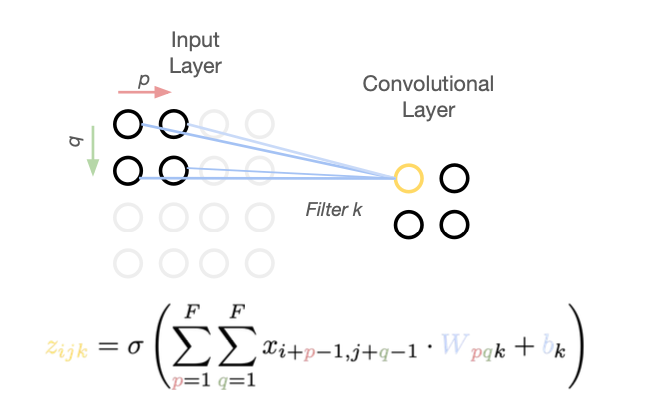
\includegraphics[width=1\textwidth]{img/4_conv.png}
    \caption{A diagram of a single convolutions filter acting on a single channel input with color- coded equation for demonstration purposes. The filter we display is two by two (or in general, $F \times F$ and the weight contributions (in blue) are multiplied by the input values (in black) and are summed over (red and green).
    }
\end{figure}

The convolutional layer is mathematically defined as:

\[
    z_{ijk} = \sigma \left( \sum_{p=1}^{F} \sum_{q=1}^{F} x_{i+p-1, j+q-1} \cdot W_{pqk} + b_k \right)
\]

Given an input \( \bm{x} \in \mathbb{R}^{H \times W \times C} \) (height \( H \), width \( W \), and \( C \) channels) and a set of \( K \) filters \( W_k \in \mathbb{R}^{F \times F \times C} \), the output feature map \( y \in \mathbb{R}^{H' \times W' \times K} \) is computed as:

\[
    y_{ijk} = \sigma \left( \sum_{c=1}^{C} \sum_{p=1}^{F} \sum_{q=1}^{F} x_{i+p-1, j+q-1, c} \cdot W_{pqck} + b_k \right)
\]

Here, \( \sigma \) is a non-linear activation function, and \( b_k \) is a bias term. The output dimensions \( H' \) and \( W' \) depend on the stride and padding used in the convolution operation. \marginnote[-100pt]{
    \noindent
    \textbf{Stride}: Stride refers to the step size with which the filter moves across the input. A larger stride reduces the spatial dimensions of the output.

    \bigskip

    \noindent
    \textbf{Padding}: Padding refers to the addition of extra pixels (typically zeros) around the input to control the output size. Padding ensures that the spatial dimensions of the input and output can be maintained or adjusted based on the chosen convolutional operation.
}

Convolutional layers are foundational in Convolutional Neural Networks (CNNs), which are widely used in tasks such as image classification, object detection, and segmentation.


\subsubsection{Recurrent Layers}

Recurrent layers are designed to handle sequential data (order of data points is important). These layers are the core components of Recurrent Neural Networks (RNNs), which are used in tasks such as time series prediction, natural language processing, and speech recognition. \bigskip

In a recurrent layer, the output at each time step depends on both the current input and the hidden state from the previous time step. This allows the network to maintain a memory of past inputs, capturing temporal dependencies.

\begin{figure}[h]
    \centering
    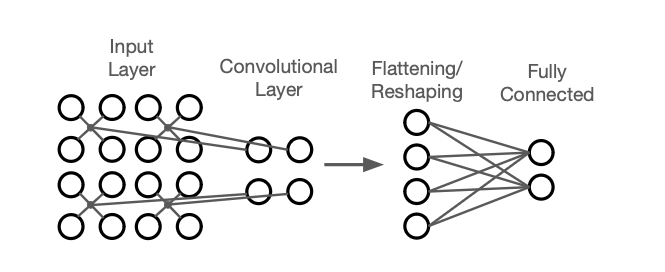
\includegraphics[width=1\textwidth]{img/4_fully_connected.png}
    \caption{A diagram of a simplistic neural network. The first layer is a convolution, followed by flattening and a fully connected layer representing the final output.}
\end{figure}

Formally, given an input sequence \( \bm{x} = [\bm{x_1}, \bm{x_2}, \dots, \bm{x_T}] \), the hidden state \( h_t \) at time step \( t \) is computed as:

\[
    h_t = \sigma \left( \bm{W}_h \bm{h}_{t-1} + \bm{W}_x \bm{x}_t + \bm{b}_h \right)
\]

where \( \bm{W}_h \) and \( \bm{W}_x \) are weight matrices, \( \bm{b}_h \) is a bias term, and \( \sigma \) is a non-linear activation function.


Variants such as Long Short-Term Memory (LSTM) networks and Gated Recurrent Units (GRUs) have been developed to address issues like vanishing gradients and to better capture long-term dependencies.


\subsubsection{Attention Layers}

Attention layers have revolutionised many areas of machine learning, particularly in natural language processing (NLP). The key idea behind attention mechanisms is to allow the model to focus on different parts of the input sequence when making predictions, rather than treating all parts of the sequence equally. This approach is a significant improvement to the model's ability to handle long sequences and complex dependencies.

\bigskip

A common type of attention mechanism is \textbf{self-attention}, where the model computes attention scores within a single sequence. Given an input sequence \( \bm{x} = [\bm{x}_1, \bm{x}_2, \dots, \bm{x}_T] \), the attention mechanism computes a set of output vectors \( \bm{y} = [\bm{y}_1, \bm{y}_2, \dots, \bm{y}_T] \) as:

\[
    \bm{y}_i = \sum_{j=1}^{T} \alpha_{ij} \bm{x}_j
\]

In this equation, \( \alpha_{ij} \) represents the attention weight that tells the model how much focus should be given to each input \( \bm{x}_j \) when generating the output \( \bm{y}_i \). The attention weights are computed using a compatibility function denoted by $a_\phi$.\bigskip

In the self-attention mechanism, the function \( a_\phi \) is used to compute the attention weights \( \alpha_{ij} \), which determine how much focus each input \( \bm{x}_j \) should receive when constructing the output \( \bm{y}_i \). \bigskip

The function \( a_\phi \) is called a compatibility function, as it measures how relevant or aligned two inputs \( \bm{x}_i \) and \( \bm{x}_j \) are. This compatibility score is then converted into a probability-like weight \( \alpha_{ij} \) through a softmax function.\bigskip

For example, in the commonly used \textbf{dot-product attention}, the function \( a_\phi \) is simply the dot product between two input vectors:
\[
    a_\phi(\bm{x}_i, \bm{x}_j) = \bm{x}_i^\top \bm{x}_j
\]
This gives a raw score of how similar or aligned \( \bm{x}_i \) and \( \bm{x}_j \) are. To compute the final attention weights \( \alpha_{ij} \), these scores are normalised across all inputs using a softmax function:
\begin{align*}
    \alpha_{ij} & = \frac{\exp(a_\phi(\bm{x}_i, \bm{x}_j))}{\sum_{k=1}^{T} \exp(a_\phi(\bm{x}_i, \bm{x}_k))}                     \\
                & = \frac{\exp \left( \bm{x}_i^\top \bm{x}_j \right)}{\sum_{k=1}^{T} \exp \left( \bm{x}_i^\top \bm{x}_k \right)}
\end{align*}

The process of computing attention scores and generating weighted sums for each output is visually depicted in Figure \ref{fig:attention}. This figure illustrates how each input vector \( \bm{e}_j \) is transformed through a function \( f_\psi \) before being scaled by attention weights \( \alpha_{ij} \). The weighted values are then summed to produce the output vector \( \bm{e}_j' \), demonstrating the flow of information in a self-attention layer.

\begin{figure}[h]
    \centering
    \begin{tikzpicture}

        \node (X1) {$\bm{x}_{1}$};
        \node[rectangle, right= 0.5em of X1] (x_dots_1) {$\dots$};
        \node[right=0.5em of x_dots_1] (Xj) {$\bm{x}_{j}$};
        \node[rectangle, right= 1em of Xj] (x_dots_2) {$\dots$};
        \node[right=1em of x_dots_2] (Xn) {$\bm{x}_{n}$};

        \node[rectangle, draw, ultra thick, above=of X1] (attn1) {\large $a_\phi$};
        \node[rectangle, draw, ultra thick, above=of Xj] (attnj) {\large $a_\phi$};
        \node[rectangle, draw, ultra thick, above=of Xn] (attnn) {\large $a_\phi$};

        \draw[-stealth, thick] (X1) -- (attn1);
        \draw[-stealth, thick] (Xj) -- (attn1);
        \draw[-stealth, thick] (Xj) -- (attnj);
        \draw[-stealth, thick] ([xshift=3em]Xj) -- (attnj);
        \draw[-stealth, thick] (Xj) -- (attnn);
        \draw[-stealth, thick] (Xn) -- (attnn);

        \node[above= of attn1, opacity=0.2] (alpha1j) {$\alpha_{1,j}$};
        \node[above= of attnj, opacity=1] (alphajj) {$\alpha_{j,j}$};
        \node[above= of attnn, opacity=0.6] (alphanj) {$\alpha_{n,j}$};

        \node[circle, draw, above=of alpha1j] (times1) {$\times$};
        \node[circle, draw, above=of alphajj] (timesj) {$\times$};
        \node[circle, draw, above=of alphanj] (timesn) {$\times$};

        \node[rectangle, draw, above=of timesj] (sum) {$\Sigma$};
        \node[above=1em of sum] (y_tprim) {$\bm{y}_i$};

        \draw[-stealth, line width=1.5mm, white] (attn1) -- (alpha1j);
        \draw[-stealth, thick, opacity=0.2] (attn1) -- (alpha1j);
        \draw[-stealth, line width=1.5mm, white] (attnj) -- (alphajj);
        \draw[-stealth, thick, opacity=1] (attnj) -- (alphajj);
        \draw[-stealth, line width=1.5mm, white] (attnn) -- (alphanj);
        \draw[-stealth, thick, opacity=0.6] (attnn) -- (alphanj);

        \draw[-stealth, white, line width=1.5mm] (X1) edge[bend right=30] (times1);
        \draw[-stealth, thick] (X1) edge[bend right=30] (times1);
        \draw[-stealth, white, line width=1.5mm] (Xj) edge[bend right=30] (timesj);
        \draw[-stealth, thick] (Xj) edge[bend right=30] (timesj);
        \draw[-stealth, thick] (Xn) edge[bend right=30] (timesn);

        \draw[-, line width=1.5mm, white] (times1) -- (sum);
        \draw[-stealth, thick] (times1) -- (sum);
        \draw[-, line width=1.5mm, white] (timesj) -- (sum);
        \draw[-stealth, thick] (timesj) -- (sum);
        \draw[-stealth, thick] (timesn) -- (sum);
        \draw[-stealth, thick] (times1) -- (sum);

        \draw[-stealth, line width=1.5mm, white] (alpha1j) -- (times1);
        \draw[-stealth, thick, opacity=0.2] (alpha1j) -- (times1);
        \draw[-stealth, line width=1.5mm, white] (alphajj) -- (timesj);
        \draw[-stealth, thick, opacity=1] (alphajj) -- (timesj);
        \draw[-stealth, line width=1.5mm, white] (alphanj) -- (timesn);
        \draw[-stealth, thick, opacity=0.6] (alphanj) -- (timesn);

        \draw[-stealth, thick] (sum) -- (y_tprim);

    \end{tikzpicture}
    \caption{Self-attention mechanism: Each input vector \( \bm{x}_j \) is weighted by attention weights \( \alpha_{ij} \) and then combined to form the output vector \( \bm{y}_i \).}
    \label{fig:attention}
\end{figure}


Self-attention is a key component of modern architectures like \textbf{Transformers} which rely heavily on this mechanism. Transformers have become state-of-the-art in many NLP tasks, such as machine translation, text generation, and question answering.


For more detailed readings, consider the seminal papers:
\begin{itemize}
    \item ``Convolutional Neural Networks for Visual Recognition" by Yann LeCun
    \item ``Long Short-Term Memory" by Hochreiter and Schmidhuber
    \item ``Attention is All You Need" by Vaswani et al.
\end{itemize}

\section{Automatic Differentiation}

In the context of Generalised Linear Models (GLMs), gradients are used for learning algorithms such as gradient descent.

\[\theta^{(t+1)}=\theta^{(t)}+\alpha\nabla_\theta\mathcal{L}(f^\theta,\bm{X},\bm{y})
\]

We will rewrite this as:

\[\theta^{(t+1)}=\theta^{(t)}-\alpha\nabla_\theta\mathcal{L}(\theta^{(t)})\]

It can sometimes be challenging to compute gradients manually. For neural networks, even small models can make manual gradient computation infeasible. To address this, we use a systematic approach called \textit{automatic differentiation}, which automates the process of computing derivatives.

\subsection{A Running Example}

Consider a one-hidden-layer neural network for regression:

\[
    \bm{z}^{(0)} = \bm{x}
\]
\[
    \zeta^{(1)} = \tanh\left( \bm{W}^{(1)} \bm{z}^{(0)} + \bm{b}^{(1)} \right)
\]
\[
    \bm{z}^{(2)} = \bm{W}^{(2)} \zeta^{(1)} + \bm{b}^{(2)}
\]

Assuming we have access to i.i.d. data samples, we aim to find parameters that minimise the loss function:
\[
    \mathcal{L}(\bm{y}, \bm{z}^{(2)}) = \left( \bm{y} - \bm{z}^{(2)} \right)^2
\]

To compute gradients such as \( \frac{\partial \mathcal{L}}{\partial \bm{W}^{(1)}} \), we would need to compute several intermediate derivatives.

\[\begin{aligned}
        \frac{\partial L}{\partial\boldsymbol{W}^{(1)}} & =\left(\frac{\partial L}{\partial\boldsymbol{z}^{(2)}}\cdot\frac{\partial\boldsymbol{z}^{(2)}}{\partial\zeta^{(1)}}\cdot\frac{\partial\zeta^{(1)}}{\partial(\boldsymbol{W}^{(1)}\boldsymbol{z}^{(0)}+\boldsymbol{b}^{(1)})}\right)\frac{\partial(\boldsymbol{W}^{(1)}\boldsymbol{z}^{(0)}+\boldsymbol{b}^{(1)})}{\partial\boldsymbol{W}^{(1)}} \\
                                                        & =\left((\boldsymbol{z}^{(2)}-\boldsymbol{y})^\top\boldsymbol{W}^{(2)}\circ\left(1-\tanh^2(\boldsymbol{W}^{(1)}\boldsymbol{z}^{(0)}+\boldsymbol{b}^{(1)})\right)\right)\boldsymbol{z}^{(0)\top}
    \end{aligned}\]

For small networks, manual computation may be feasible, but for deeper models, this process becomes impractical. Plus, everytime we make a minor modification we would need to re-derive our gradients. \bigskip

An alternative method to compute derivatives is the\textbf{ finite difference approach,} which approximates the derivative of a function \( f : \mathbb{R}^n \to \mathbb{R} \). For each input \( x_i \), the partial derivative can be approximated by:

\[
    \frac{\partial f}{\partial x_1} = \lim_{h \to 0} \frac{f(x_1 + h, x_2, \dots, x_n) - f(x_1, x_2, \dots, x_n)}{h}
\]
\[
    \frac{\partial f}{\partial x_2} = \lim_{h \to 0} \frac{f(x_1, x_2 + h, \dots, x_n) - f(x_1, x_2, \dots, x_n)}{h}
\]
\[
    \vdots
\]
\[
    \frac{\partial f}{\partial x_n} = \lim_{h \to 0} \frac{f(x_1, x_2, \dots, x_n + h) - f(x_1, x_2, \dots, x_n)}{h}
\]

The complexity of this method is $O(2nT)$, where $n$ is the number of parameters and $T$ is the complexity of evaluating the function or model once. We evaluate the function twice at $\bm{x}$ and $\bm{x} + (\bm{1} \cdot h)$ for $n$ parameters.\bigskip

However, applying this method to each parameter can be cumbersome and prone to compounded approximation errors, particularly in high-dimensional settings or complex functions.


\subsection{Introducing Automatic Differentiation}



The main concept of automatic differentiation is to break down complex equations into simpler operations, each of which can be easily differentiated. We can then apply the chain rule systematically. By understanding the sequence of operations, we can express the overall model as a composition of functions:
\[
    f(\bm{x}) = h(g(\bm{x}))
\]

\marginnote{

    \sns{Side Note on AutoDiff}{

        We are trying to compute $\alpha \nabla_{\theta} \mathcal{L}(\theta^{(t)})$ in
        \[
            \theta^{(t+1)} = \theta^{(t)} - \alpha \nabla_{\theta} \mathcal{L}(\theta^{(t)})
        \]
        \(\bm{J} := \nabla_{\theta} \mathcal{L}(\theta) \in \mathbb{R}^{m \times n}\),\\
        \(\theta^{(t)} \in \mathbb{R}^{n \times 1}\),\\
        \(\mathcal{L}(\theta) : \mathbb{R}^n \rightarrow \mathbb{R}^m\),\\
        \(\alpha > 0\),\\


    }

}

Previously, we sought an analytical expression for the Jacobian matrix, \( \nabla_x f \), to solve for optimal parameters. Consider two functions \( g: \mathbb{R}^n \to \mathbb{R}^k \) and \( h: \mathbb{R}^k \to \mathbb{R}^m \). By applying the chain rule, the Jacobian of the composed function is given by:

\[
    \bm{J}_f = \bm{J}_{h \circ g} = \bm{J}_h(g(\bm{x})) \bm{J}_g(\bm{x})
\]

This general principle allows us to compute \textbf{directional derivatives}, which are used to assemble gradients. Given a series of \( L \) compositions of functions, the directional derivative computed via automatic differentiation is:

\[
    \bm{J} \bm{x} = \bm{J}^{(L)} \bm{J}^{(L-1)} \dots \bm{J}^{(1)} \bm{x}
\]

Here, we are not computing the full Jacobian matrix, but rather the \textbf{Jacobian-vector product} with respect to the vector \( \bm{x} \), which is referred to as the \textbf{directional }derivative.

\subsection{Forward-Mode Automatic Differentiation}

The first paradigm of automatic differentiation we will cover is forward-mode. The key idea is that we compute the necessary derivatives of our function concurrently with the values during the forward pass. Forward mode can be viewed as breaking down the Jacobian-vector product in a sequential manner, as shown below:

\begin{align}
    \bm{J} \bm{x} & = \bm{J}^{(L)} \bm{J}^{(L-1)} \dots \bm{J}^{(1)} \bm{x} \notag                      \\
                  & = \bm{J}^{(L)} \bm{J}^{(L-1)} \dots \bm{J}^{(2)} (\bm{J}^{(1)} \bm{x}^{(1)}) \notag \\
                  & = \bm{J}^{(L)} \bm{J}^{(L-1)} \dots \bm{J}^{(3)} (\bm{J}^{(2)} \bm{x}^{(2)}) \notag \\
                  & \dots \notag                                                                        \\
    \bm{J} \bm{x} & = \bm{J}^{(L)} \bm{x}^{(L-1)} \label{eq:forward-mode-jacobian}
\end{align}


Here, \( \bm{x}^{(L-1)} \) denotes the intermediate result after the last Jacobian has been applied. \bigskip

Now, let us apply this process to a simple neural network model. In practice, when training neural networks, we aim to compute the gradient with respect to the parameters. However, to demonstrate the forward-mode process, we will compute the input gradient step by step. First, recall our example:

\[
    \bm{z}^{(0)} = \bm{x}
\]
\[
    \zeta^{(1)} = \tanh\left( \bm{W}^{(1)} \bm{z}^{(0)} + \bm{b}^{(1)} \right)
\]
\[
    \bm{z}^{(2)} = \bm{W}^{(2)} \zeta^{(1)} + \bm{b}^{(2)}
\]


Then, we express the forward pass and the loss function as a sequence of functions that we can program:

\begin{equation}
    \bm{z}^{(2)} = \text{Matmul}\left( \bm{W}^{(1)}, \tanh\left( \text{Matmul} \left( \bm{W}^{(0)} \bm{z}^{(0)} \right) \right) \right)
\end{equation}
\begin{equation}
    \mathcal{L} = \left( \bm{y} - \bm{z}^{(2)} \right)^2
\end{equation}

The purpose of this step is to identify the elementary operations involved in computing the loss, which will help us build the computational graph. \bigskip

In automatic differentiation literature, these operations are referred to as \textbf{primitives}. Each primitive represents a basic operation that is easy to differentiate. For example, the primitives we commonly deal with include functions like addition, multiplication, or applying activation functions (like \( \tanh \) or raising to a power). For each primitive, the differentiation rules from calculus apply.


\begin{figure}[ht]
    \centering
    \begin{tabularx}{\linewidth}{p{0.2\linewidth} p{0.2\linewidth} p{0.6\linewidth}}
        \toprule
        \textbf{Operation}               & \textbf{Value Update} & \textbf{Derivative Update}                                       \\
        \midrule
        Addition of a constant $c$       & $g(w) + c$            & $\frac{d}{dw}(g(w) + c) = \frac{d}{dw}g(w)$                      \\
        \hline
        Multiplication by a constant $c$ & $cg(w)$               & $\frac{d}{dw}(cg(w)) = c \frac{d}{dw}g(w)$                       \\
        \hline
        Raising to a power $n$           & $g(w)^n$              & $\frac{d}{dw}(g(w)^n) = n(g(w)^{n-1})\frac{d}{dw}g(w)$           \\
        \hline
        Applying Tanh                    & $\tanh(g(w))$         & $\frac{d}{dw}(\tanh(g(w))) = 1 - \tanh^2(g(w)) \frac{d}{dw}g(w)$ \\
        \bottomrule
    \end{tabularx}
    \caption{Value and Derivative Updates for Various Operations}
\end{figure}

Returning to our equations– we ignore the bias terms because they are relegated to affine basis expansion for brevity. We can now compute the forward pass and the derivative of the loss function, step by step:

\begin{align*}
    \bm{z}^{(0)} & = \bm{x}                                                                                                               \\
    \zeta^{(1)}  & = \tanh\left( \bm{W}^{(1)} \bm{z}^{(0)} + \bm{b}^{(1)} \right)                                                         \\
    \bm{z}^{(2)} & = \bm{W}^{(2)} \zeta^{(1)} + \bm{b}^{(2)}                                                                              \\
                 & = \text{Matmul}\left( \bm{W}^{(1)}, \tanh\left( \text{Matmul} \left( \bm{W}^{(0)} \bm{z}^{(0)} \right) \right) \right) \\
    \mathcal{L}  & = \left( \bm{y} - \bm{z}^{(2)} \right)^2
\end{align*}

\begin{figure}[h!]
    \centering
    \begin{tabularx}{\linewidth}{X X}
        \toprule
        \textbf{Value}      & \textbf{Derivative}          \\
        \midrule
        $x_0 = x$           & $d_0 = \bm{1}$               \\
        $x_1 = W^{(0)} x_0$ & $d_1 = W^{(0)\top} d_0$      \\
        $x_2 = \tanh(x_1)$  & $d_2 = 1 - \tanh^2(x_1) d_1$ \\
        $x_3 = W^{(1)} x_2$ & $d_3 = W^{(1)\top} d_2$      \\
        $x_4 = (y - x_3)$   & $d_4 = -d_3$                 \\
        $x_5 = (x_4)^2$     & $d_4 = 2(x_4) d_4$           \\
        \bottomrule
    \end{tabularx}
    \caption{Forward and Backward Pass for Value and Derivative Calculation. }
\end{figure}

\begin{figure}[h!]
    \centering
    \begin{tikzpicture}[>=Stealth, node distance=0.5cm, auto, scale=0.9, transform shape]
        % Define styles for nodes
        \tikzset{
            op/.style={rectangle, draw=black, fill=blue!20, thick, minimum size=8mm, rounded corners},
            var/.style={circle, draw=black, fill=yellow!30, thick, minimum size=8mm},
            arrow/.style={->, thick}
        }

        % Nodes for forward pass
        \node[var] (x0) {$x$};
        \node[var] (y) [below=of x0] {$y$};
        \node[op, right=of x0] (w0x0) {$\text{Matmul}\left(\bm{W}^{(0)} ( \cdot)\right)$};
        \node[var, right=of w0x0] (x1) {$x_1$};
        \node[op, right=of x1] (tanh1) {$\tanh(\cdot)$};
        \node[var, right=of tanh1] (x2) {$x_2$};
        \node[op, right=of x2] (w1x2) {$\text{Matmul}\left(\bm{W}^{(1)} ( \cdot)\right)$};
        \node[var, below=of w1x2] (x3) {$x_3$};
        \node[op, left=of x3] (sub) {$-$};
        \node[var, below=of sub] (x4) {$x_4$};
        \node[op, left=of x4] (square) {$(\cdot)^2$};
        \node[var, left=of square] (L) {$\mathcal{L}$};

        % Edges for forward pass
        \draw[arrow] (x0) -- (w0x0);
        \draw[arrow] (w0x0) -- (x1);
        \draw[arrow] (x1) -- (tanh1);
        \draw[arrow] (tanh1) -- (x2);
        \draw[arrow] (x2) -- (w1x2);
        \draw[arrow] (w1x2) -- (x3);
        \draw[arrow] (x3) -- (sub);
        \draw[arrow] (sub) -- (x4);
        \draw[arrow] (x4) -- (square);
        \draw[arrow] (square) -- (L);
        \draw[arrow] (y) -- (sub);

        % % Backward pass (derivatives)
        % \node[var, below=3.0cm of w1x2, ] (d4) {$d_4$};
        % \node[op, left=of d4] (subd3) {$-$};
        % \node[var, left=of subd3] (d3) {$d_3$};
        % \node[op, left=of d3] (tanhd2) {$1-\tanh^2$};
        % \node[var, left=of tanhd2] (d2) {$d_2$};
        % \node[op, left=of d2] (w0td1) {$W^{(0)\top}$};
        % \node[var, left=of w0td1] (d1) {$d_1$};
        % \node[op, left=of d1] (loss) {Loss};

        % % Edges for backward pass
        % \draw[arrow] (d4) -- (subd3);
        % \draw[arrow] (subd3) -- (d3);
        % \draw[arrow] (d3) -- (tanhd2);
        % \draw[arrow] (tanhd2) -- (d2);
        % \draw[arrow] (d2) -- (w0td1);
        % \draw[arrow] (w0td1) -- (d1);
        % \draw[arrow] (d1) -- (loss);
    \end{tikzpicture}
    \caption{Computational Graph for the example neural network.}
\end{figure}

For an example $x = 1$, $W^{(0)} = 2$, $W^{(1)} = 1.2$, $y = 2$, the calculations would look like the following:
\begin{figure}[h!]
    \centering
    \begin{tabularx}{\linewidth}{p{0.4\linewidth} p{0.6\linewidth}}
        \toprule
        \textbf{Value}                                                & \textbf{Derivative}                                                   \\
        \midrule
        $x_0 = x \Rightarrow 1$                                       & $d_0 = \bm{1}$                                                        \\
        $x_1 = W^{(0)} x_0 \Rightarrow 1 \times 2 = 2$                & $d_1 = W^{(0)\top} d_0 \Rightarrow 2 \times d_0 = 2$                  \\
        $x_2 = \tanh(x_1) \Rightarrow \tanh(2) \approx 0.964$         & $d_2 = (1 - \tanh^2(2)) d_1 \Rightarrow 0.14 \times d_1 \approx 0.14$ \\
        $x_3 = W^{(1)} x_2 \Rightarrow 1.2 \times 0.964 \approx 1.15$ & $d_3 = W^{(1)\top} d_2 \Rightarrow 1.2 \times 0.14 \approx 0.169$     \\
        $x_4 = y - x_3 \Rightarrow 2 - 1.15 = 0.85$                   & $d_4 = -d_3 \Rightarrow -0.169$                                       \\
        $x_5 = (x_4)^2 \Rightarrow (0.85)^2 = 0.722$                  & $d_5 = 2(x_4) d_4 \Rightarrow 2(0.85) \times (-0.169) \approx -0.283$ \\
        \bottomrule
    \end{tabularx}
    \caption{Forward and Backward Pass for Value and Derivative Calculation with extensions.}
\end{figure}


To clarify, \( \bm{x}_0 \) is the input, \( \bm{x}_1 \) is the result of the first matrix multiplication, \( \bm{x}_2 \) is after applying the activation function, \( \bm{x}_3 \) is the second matrix multiplication, \( \bm{x}_4 \) represents the absolute error with respect to the label, and \( \bm{x}_5 \) is the squared error. We computed \( d_5 = \frac{d \mathcal{L}}{d \bm{x}} = -0.283 \), but this does not provide \( \frac{d \mathcal{L}}{d \bm{W}^{(1)}} \). To compute this, another forward differentiation would be needed, which is beyond this example.


\subsection{Complexity of Forward Mode Differentiation}

Let the forward pass complexity be $T$, the number of operations required to compute the function. The computational complexity of finding the Jacobian with forward mode automatic differentiation is $O(2nT)$. This is identical to the complexity of finite-difference approximation, but a much less approximation error since approximations are not compounded.

\subsection{Reverse-Mode Automatic Differentiation}

The idea of reverse mode is to begin with an output and propagate backwards, rather than beginning with an input and propagating forwards. This is particularly useful when the number of inputs is much larger than the number of outputs, as is the case with neural networks. \bigskip

In forward-mode automatic differentiation (AD), we track both the nominal values and the tangents (directional derivatives). We could do this by using the associativity of matrix products that give us our Jacobian matrix, as in Equation \ref{eq:forward-mode-jacobian}. \bigskip

Reverse-mode AD, however, focuses on computing adjoints, which can be defined as:
\[
    \bar{x} = \frac{\partial z}{\partial x}
\]

\defb{`Adjoint' in Automatic Differentiation (AD)}{
    `Adjoint' comes from linear algebra, and in the context of automatic differentiation (AD), particuarly reverse-mode AD, it refers to the propagation of derivatives. \bigskip

    The adjoint of a variable $x$ is the derivative of the target function (often the loss function in ML) with respect to $x$. It is framed towards the reverse accumulation of derivatives in a system.


    \[
        \bar{x} = \frac{\partial z}{\partial x}
    \]
}

This adjoint must have the correct shape to be multiplied by the Jacobian. To illustrate, consider the output of a model, \( \bm{y} - f(\bm{x}) \), and compute the derivative in reverse order with respect to the output:



\begin{align*}
    \bm{Jx} = \bar{\bm{y}} \bm{J} & = (\bar{\bm{y}} \bm{J}^{(L)}) \bm{J}^{(L-1)} \dots \bm{J}^{(1)}           \\
                                  & = (\bar{\bm{y}}^{(L)} \bm{J}^{(L-1)}) \bm{J}^{(L-2)} \dots \bm{J}^{(1)}   \\
                                  & = (\bar{\bm{y}}^{(L-1)} \bm{J}^{(L-2)}) \bm{J}^{(L-3)} \dots \bm{J}^{(1)} \\
                                  & \dots                                                                     \\
                                  & = \bar{\bm{y}}^{(2)} \bm{J}^{(1)}
\end{align*}

\marginnote[-80pt]{

    \sns{Side Note on AutoDiff}{

        We are trying to compute $\alpha \nabla_{\theta} \mathcal{L}(\theta^{(t)})$ in
        \[
            \theta^{(t+1)} = \theta^{(t)} - \alpha \nabla_{\theta} \mathcal{L}(\theta^{(t)})
        \]
        \(\bm{J} := \nabla_{\theta} \mathcal{L}(\theta) \in \mathbb{R}^{m \times n}\),\\
        \(\theta^{(t)} \in \mathbb{R}^{n \times 1}\),\\
        \(\mathcal{L}(\theta) : \mathbb{R}^n \rightarrow \mathbb{R}^m\),\\
        \(\alpha > 0\),\\


    }

    In contrast to Forward Mode:

    \begin{align*}
        \bm{J} \bm{x} & = \bm{J}^{(L)} \bm{J}^{(L-1)} \dots \bm{J}^{(1)} \bm{x}                      \\
                      & = \bm{J}^{(L)} \bm{J}^{(L-1)} \dots \bm{J}^{(2)} (\bm{J}^{(1)} \bm{x}^{(1)}) \\
                      & = \bm{J}^{(L)} \bm{J}^{(L-1)} \dots \bm{J}^{(3)} (\bm{J}^{(2)} \bm{x}^{(2)}) \\
                      & \dots                                                                        \\
        \bm{J} \bm{x} & = \bm{J}^{(L)} \bm{x}^{(L-1)}
    \end{align*}

}



In reverse mode, we compute the necessary Jacobians in reverse order, meaning we need intermediate results from the forward pass. For a fully connected neural network with \( L \) layers, the forward pass is given by:

\begin{align*}
    \bm{z}^{(1)}   & = \bm{x}                                                        \\
    \bm{z}^{(i+1)} & = \sigma\left( \bm{W}^{(i)} \bm{z}^{(i)} + \bm{b}^{(i)} \right)
\end{align*}

Now, let us consider the weights and biases to be joined into parameters denoted \( \theta^{(i)} = \{ \bm{W}^{(i)}, \bm{b}^{(i)} \} \). We aim to compute the gradient of our function starting from the last layer using the chain rule:

\begin{align*}
    \frac{\partial \mathcal{L}}{\partial \theta^{(L-1)}} & = \frac{\partial \mathcal{L}}{\partial \bm{z}^{(L)}} \textcolor{blue}{\frac{\partial \bm{z}^{(L)}}{\partial \theta^{(L-1)}}}                                                                                                                                                                                                                \\
    \frac{\partial \mathcal{L}}{\partial \theta^{(L-2)}} & = \frac{\partial \mathcal{L}}{\partial \bm{z}^{(L)}} \textcolor{orange}{\frac{\partial \bm{z}^{(L)}}{\partial \bm{z}^{(L-1)}}} \textcolor{blue}{\frac{\partial \bm{z}^{(L-1)}}{\partial \theta^{(L-2)}}}                                                                                                                                    \\
    \frac{\partial \mathcal{L}}{\partial \theta^{(L-3)}} & = \frac{\partial \mathcal{L}}{\partial \bm{z}^{(L)}} \textcolor{orange}{\frac{\partial \bm{z}^{(L)}}{\partial \bm{z}^{(L-1)}} \frac{\partial \bm{z}^{(L-1)}}{\partial \bm{z}^{(L-2)}} } \textcolor{blue}{\frac{\partial \bm{z}^{(1)}}{\partial \theta^{(L-3)}}}                                                                             \\
    \frac{\partial \mathcal{L}}{\partial \theta^{(i)}}   & = \frac{\partial \mathcal{L}}{\partial \bm{z}^{(L)}} \textcolor{orange}{\frac{\partial \bm{z}^{(L)}}{\partial \bm{z}^{(L-1)}} \frac{\partial \bm{z}^{(L-1)}}{\partial \bm{z}^{(L-2)}} } \dots \textcolor{orange}{\frac{\partial \bm{z}^{(2)}}{\partial \bm{z}^{(1)}}} \textcolor{blue}{\frac{\partial \bm{z}^{(1)}}{\partial \theta^{(i)}}}
\end{align*}

We can observe that by chain rule, we can compute the partial derivative of the parameters in layer $i$ by computing the \textcolor{orange}{partial derivative of the layer w.r.t its input}, and then multiply it with the \textcolor{blue}{partial derivative of the layer output w.r.t its parameters}. Using this recursive application of the chain rule, we propagate the error back through the layers, computing the gradient of the loss \( \mathcal{L} \) with respect to each parameter \( \theta^{(i)} \).

\newpage
\subsection{General Adjoint/Reverse Mode Algorithm}

We now describe the general reverse-mode automatic differentiation algorithm. Let \( x_1, x_2, \dots, x_D \) be the input variables, and \( x_{d+1}, \dots, x_{D-1} \) be the intermediate variables, with \( x_D \) as the output variable. The flow of the computational graph is given by: \marginnote{
    We are trying to avoid graph theory notation as much as possible in the notes.
}

\begin{equation}
    x_i = g_i(x_{\text{Pa}(x_i)})
    \quad \forall i \in [d+1, D]
\end{equation}

Here, \( g_i \) is the elementary operation associated with the node in the graph, and \( \text{Pa}(x_i) \) is the function that returns the set of parent (incoming) nodes to variable \( x_i \).


\begin{figure}[h!]
    \centering
    \begin{tikzpicture}[>=Stealth, node distance=0.5cm, auto, scale=0.9, transform shape]
        % Define styles for nodes
        \tikzset{
            op/.style={rectangle, draw=black, fill=blue!20, thick, minimum size=13mm, rounded corners},
            var/.style={circle, draw=black, fill=yellow!30, thick, minimum size=13mm},
            arrow/.style={->, thick}
        }

        % Input Nodes
        \node[var] (x1) {$x_1$};
        \node[var, below= of x1] (x2) {$x_2$};
        \node[draw=none, below= of x2] (xdots) {$\vdots$};
        \node[var, below= of xdots] (xd) {$x_d$};

        % Operations
        \node[op, right=of x1] (gd1) {$g_{d+1}$};
        \node[op, right=of x2] (gd2) {$g_{d+2}$};
        \node[draw=none, below=of gd2] (xdots) {$\vdots$};


        % Intermediate Nodes
        \node[var, right=of gd1] (xd1) {$x_{d+1}$};
        \node[var, right=of gd2] (xd2) {$x_{d+2}$};
        \node[draw=none, below=of xd2] (xdots) {$\vdots$};

        % Operations
        \node[op, right=2cm of xd1] (gd3) {$g_{D}$};
        \node[draw=none, right=of xd1, yshift=0.1cm] (gdots) {$\cdots$};

        % Last Nodes
        \node[var, right=of gd3] (xD) {$x_{D}$};


        % Intermediate and output nodes
        % Output node
        % \node[var, right=of g4] (output) {$f$};

        \draw[arrow] (x1) -- (gd1.west);
        \draw[arrow] (x2) -- (gd2.west);
        \draw[arrow] (xd) -- (gd1.west);

        \draw[arrow] (xd) -- (gd2.west);

        \draw[arrow] (gd1) -- (xd1.west);
        \draw[arrow] (gd2) -- (xd2.west);

        \draw[arrow] (xd1) -- (gd3.west);
        \draw[arrow] (xd2) -- (gd3.west);

        \draw[arrow] (xd) to[bend right] (gd3.south);
        \draw[arrow] (gd3) -- (xD.west);






    \end{tikzpicture}
    \caption{Computational Graph notation}
\end{figure}


The chain rule can then be applied to compute the derivative:

\defb{
    Reverse Mode
}
{
    \begin{equation}
        \frac{\partial f}{\partial x_i} = \sum_{x_j : i \in \text{Pa}(x_j)} \frac{\partial x_j}{\partial x_i} \frac{\partial f}{\partial x_j} = \sum_{x_j : i \in \text{Pa}(x_j)} \frac{\partial g_j}{\partial x_i} \frac{\partial f}{\partial x_j} \label{eq:reverse-mode-chain-rule}
    \end{equation}
}



\ex{Example of finding the computational graph}{
Consider the function:

\[
    f(x) = \sqrt{x^2 + \exp(x^2)} + \cos\left( x^2 + \exp(x^2) \right)
\]

We break this equation down into its elementary operations: { square root, exponential, power, cosine, addition }:

\begin{align*}
    x_1 & = x^2 \quad        & \frac{\partial x_1}{\partial x}   & = 2x                                   \\
    x_2 & = \exp(x_1) \quad  & \frac{\partial x_2}{\partial x_1} & = \exp(x_1)                            \\
    x_3 & = x_1 + x_2 \quad  & \frac{\partial x_3}{\partial x_1} & =\frac{\partial x_3}{\partial x_2} = 1 \\
    x_4 & = \sqrt{x_3} \quad & \frac{\partial x_4}{\partial x_3} & = \frac{1}{2\sqrt{x_3}}                \\
    x_5 & = \cos(x_3) \quad  & \frac{\partial x_5}{\partial x_3} & = -\sin(x_3)                           \\
    x_6 & = x_4 + x_5 \quad  & \frac{\partial x_6}{\partial x_4} & =\frac{\partial x_6}{\partial x_5} = 1
\end{align*}

Here, \( x_6 \) represents the complete function \( f(z) \). Before performing the backward pass, it is useful to write out the derivative of each function at each step.

\begin{center}
    \begin{tikzpicture}[>=Stealth, node distance=0.5cm, auto, scale=0.85, transform shape]
        % Define styles for nodes
        \tikzset{
            op/.style={rectangle, draw=black, fill=blue!20, thick, minimum size=8mm, rounded corners},
            var/.style={circle, draw=black, fill=yellow!30, thick, minimum size=8mm},
            arrow/.style={->, thick}
        }

        % Nodes for the graph
        \node[var] (x) {$x$};
        \node[op, right=of x] (square) {$(\cdot)^2$};
        \node[var, right=of square] (a) {$x_1$};
        \node[op, above right=of a] (exp) {exp$(\cdot)$};
        \node[var, right=of exp] (b) {$x_2$};
        \node[op, below right=of b] (plus1) {$+$};
        \node[var, right=of plus1] (c) {$x_3$};
        \node[op, above right=of c] (sqrt) {$\sqrt{\cdot}$};
        \node[var, right=of sqrt] (d) {$x_4$};
        \node[op, below right=of c] (cos) {cos$(\cdot)$};
        \node[var, right=of cos] (e) {$x_5$};
        \node[op, below right=of d] (plus2) {$+$};
        \node[var, right=of plus2] (f) {$f$};

        % Edges for the graph
        \draw[arrow] (x) -- (square);
        \draw[arrow] (square) -- (a);
        \draw[arrow] (a) to[bend left] (exp.west);
        \draw[arrow] (exp.east) -- (b);
        \draw[arrow] (b) to[bend left] (plus1.north);
        \draw[arrow] (a) -- (plus1);
        \draw[arrow] (plus1) -- (c);
        \draw[arrow] (c) to[bend left] (sqrt.west);
        \draw[arrow] (sqrt) -- (d);
        \draw[arrow] (d) to[bend left] (plus2.north);
        \draw[arrow] (c) to[bend right] (cos.west);
        \draw[arrow] (cos) -- (e);
        \draw[arrow] (e) to[bend right] (plus2.south);
        \draw[arrow] (plus2) -- (f);


    \end{tikzpicture}
\end{center}

Now that we have defined the derivatives, we can construct a computational graph by working backwards from the output. The chain rule is applied step by step:

\begin{align*}
    \frac{\partial x_6}{\partial x_3} & = \frac{\partial x_6}{\partial x_4} \frac{\partial x_4}{\partial x_3} + \frac{\partial x_6}{\partial x_5} \frac{\partial x_5}{\partial x_3} \\
    \frac{\partial x_6}{\partial x_2} & = \frac{\partial x_6}{\partial x_3} \frac{\partial x_3}{\partial x_2}                                                                       \\
    \frac{\partial x_6}{\partial x_1} & = \frac{\partial x_6}{\partial x_2} \frac{\partial x_2}{\partial x_1} + \frac{\partial x_6}{\partial x_3} \frac{\partial x_3}{\partial x_1} \\
    \frac{\partial x_6}{\partial x}   & = \frac{\partial x_6}{\partial x_1} \frac{\partial x_1}{\partial x}
\end{align*}

While working backwards, ensure all parent nodes are accounted for (summed) to avoid incorrect partial derivatives. Though we only derive the recipe for the derivative and not the actual values, understanding the process outlined in Equations \ref{eq:forward-mode-jacobian} is important.



}

\subsection{Complexity of Reverse Mode Differentiation}
\begin{itemize}
    \item The function must be evaluated once(forward pass) to get the output, in order to compute all the intermediate values. This has complexity $T$.
    \item The function must be evaluated (with complexity $T$) for each of the $m$ outputs.
    \item We get $O(mT + T)$. In many cases, $m$ is much smaller than the number of inputs, so reverse mode (with complexity $O(mT+T)$) is more efficient than forward mode (with complexity $O(2nT)$).
\end{itemize}
